\begin{Exercise}
In this exercise we will create simple circuits that illustrate the concept of lateral inhibition, which is the 
capacity of an excited neuron to reduce the activity of its neighbors. This type of inhibition occurs primarily in 
visual processes to increase the sharpness in visual response.

\Question{Create a circuit in Neuronify consisting of two passive excitatory neuron and one passive inhibitory neuron, 
each 
connected to the same DC clamp. Adjust the current output of the DC clamp and see how the spiking pattern of the 
neurons changes.}

\Question{Create lateral connections from the inhibitory neuron to the excitatory neurons. How does these 
connections affect the activity in the excitatory neurons?}
   
\Question{Make the connections in the network shown below such that the spiking pattern is the same as in the 
figure. You are allowed to adjust the 
\emph{stimulation output} property of the cells and use DC clamp with different current output for the upper neurons.}
      

\Question{The network you have created now is an example where sharpening of the signal occurs through lateral 
inhibition. 
How those 
the relative strength of the inputs to the upper neurons affect the spiking of the lowermost neurons?}

\Question{Does the lateral inhibition circuit increase or decrease the contrast between strong and weak signals?}

\end{Exercise}

    
\begin{figure}[h!]
  \centering
    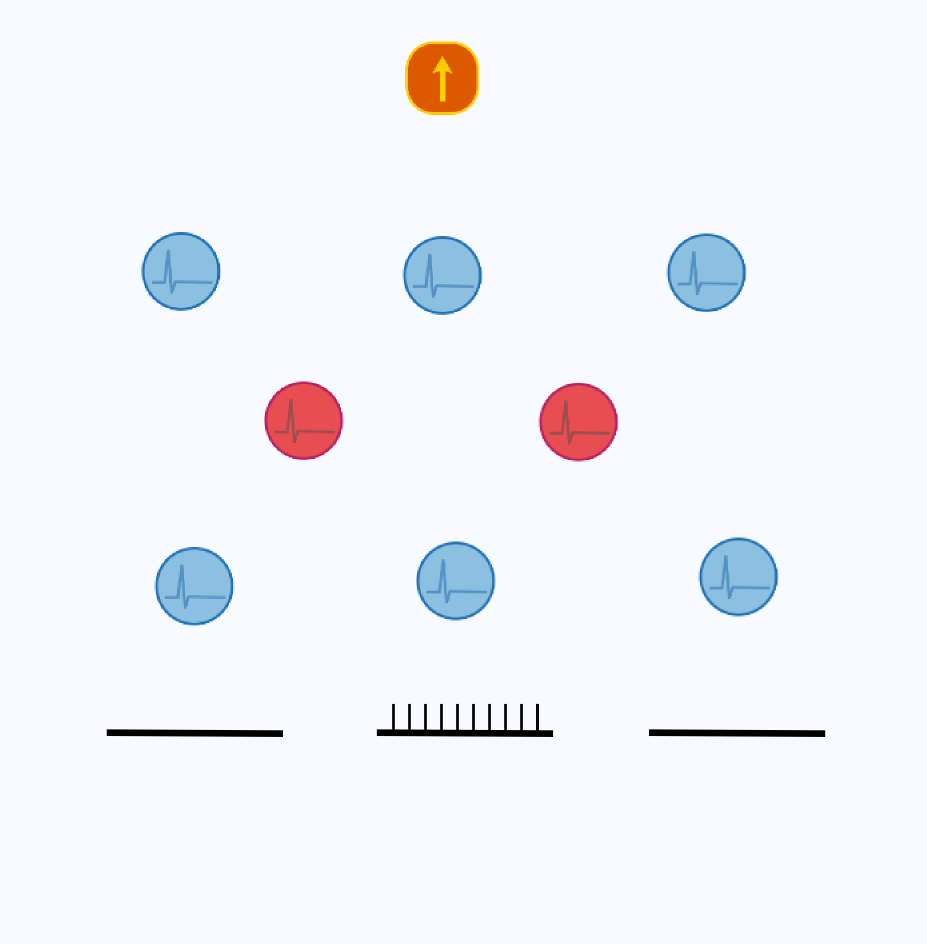
\includegraphics[width=0.5\textwidth]{figures/lateralInihibition.png}
      \caption{Lateral inhibition network.}
\end{figure}